% !TEX root = main.tex
\section{Fuja dos Juros (e das dívidas)} \label{FormProb}

\begin{frame}[c]
    \frametitle{}
    \begin{columns}
        \begin{column}{0.5\textwidth}
            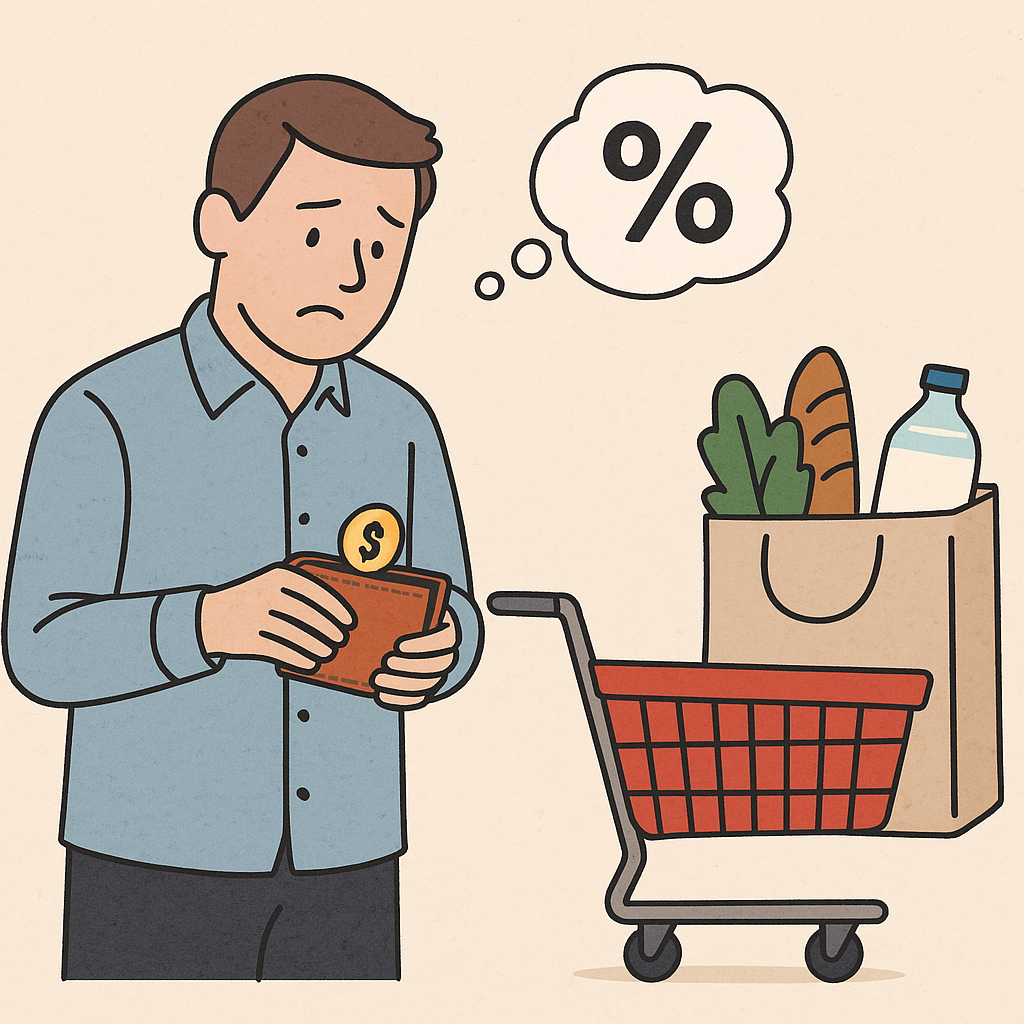
\includegraphics[width=\textwidth]{../figuras/consumo2.png}
        \end{column}
        \begin{column}{0.5\textwidth}
            \centering
            \begin{itemize}
                \item Juros é o aluguel do dinheiro.
                \item Geralmente é usado para antecipar um consumo.
                \item Comprar com juros é pagar mais caro pelo mesmo produto.
                \item Quem paga juros reduz seu poder de consumo.
            \end{itemize}
            % \textbf{\Large Juros é o aluguel do dinheiro}
        \end{column}
    \end{columns}
\end{frame}

% \begin{frame}[c]
%     \frametitle{}
%     \begin{columns}
%         \begin{column}{0.5\textwidth}
%             
\includegraphics[width=\textwidth]{../figuras/consumo3.png}
%         \end{column}
%         \begin{column}{0.5\textwidth}
%             \centering
%             \textbf{\Large Comprar com juros é pagar mais caro pelo mesmo produto.}
%         \end{column}
%     \end{columns}
% \end{frame}

% \begin{frame}[c]
%     \frametitle{}
%     \begin{columns}
%         \begin{column}{0.5\textwidth}
%             \centering
%             \textbf{\Large Quem paga juros reduz seu poder de consumo.}
%         \end{column}
%         \begin{column}{0.5\textwidth}
%             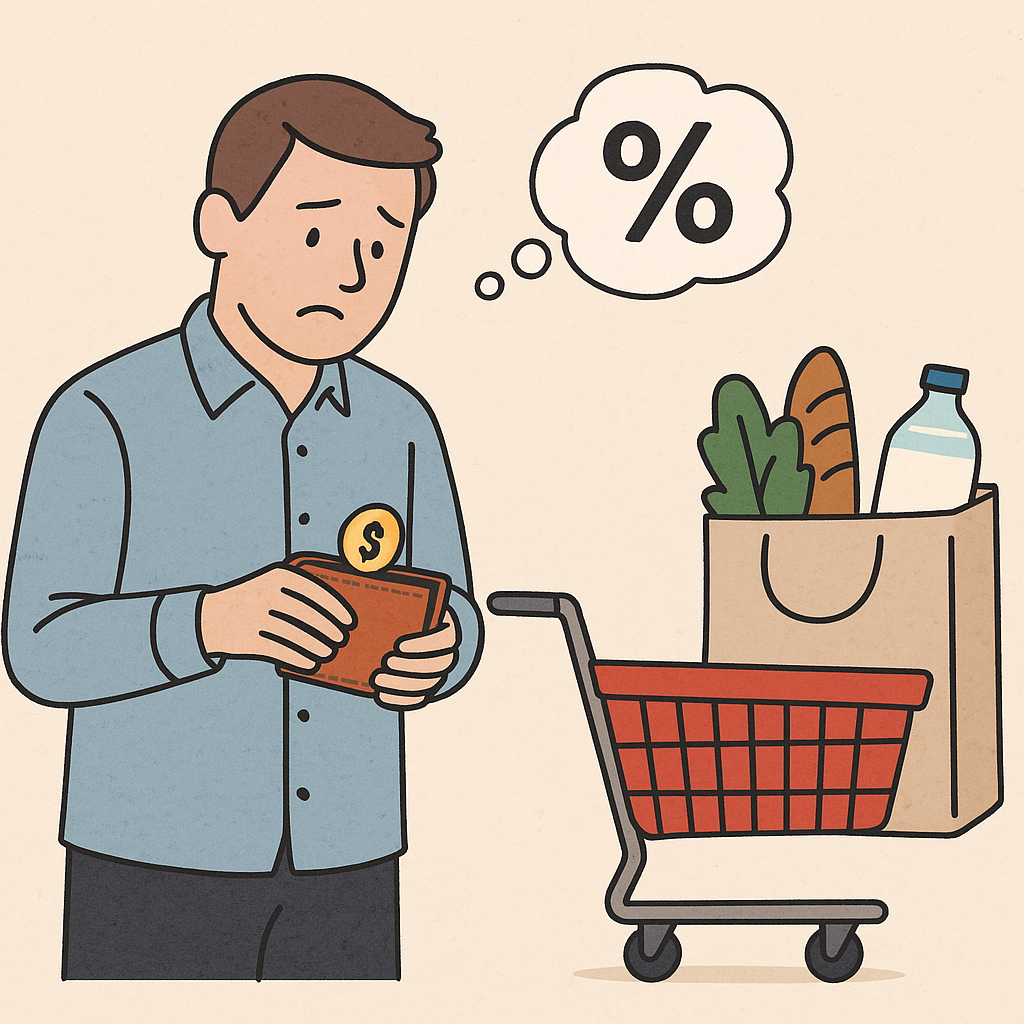
\includegraphics[width=\textwidth]{../figuras/consumo2.png}
%         \end{column}
%     \end{columns}
% \end{frame}


% \begin{frame}[c]\frametitle{Podemos alugar nosso dinheiro para}
%     % \textbf{Minha Estratégia para quitar as dívidas}
%     \begin{itemize}
%         \item Bancos através de CDB, LCI, LCA, etc.
%         \item Governo através dos títulos do Tesouro Direto.
%         \item Empresas através de Debêntures.
%     \end{itemize}
% \end{frame}

\section{Quite suas dívidas primeiro}

\begin{frame}[c]\frametitle{Estratégia para quitar as dívidas e liberar o orçamento}
    \textbf{Plano de Ação}
    \begin{itemize}
        \item \textbf{Crie um Orçamento:} Ajuste seus gastos para que sejam sempre menores do que o seu ganho mensal.
        \item \textbf{Use Rendas Extras:} Direcione o 13$^\text{o}$ salário, adicional de férias e outros bônus exclusivamente para o pagamento das dívidas.
        \item \textbf{Busque Renda Extra:} Aumente sua receita mensal com trabalhos adicionais para acelerar a quitação.
        \item \textbf{Controle a Inflação do Estilo de Vida:} Não aumente seus gastos ao receber um aumento salarial. Use o valor extra para pagar as dívidas ou para investir.
    \end{itemize}
\end{frame}